\chapter{関連技術}
\label{chap:related_works}

本章では,本研究における手法を選ぶに当たって,既存の基盤手法の比較と,基盤技術として使用するRDMA(Remote Direct Memory Address)に関して述べる.

\section{オペレーティングシステム解析手段}

本セクションでは,\ref{chap:introduction}で述べた,既存のオペレーティングシステムおよびプロセスの解析技術について述べる.
コアダンプを用いた静的解析や,kgdb,VMを用いた解析に関して述べた後,その手法の一つであるlibvmiについて述べる.

\subsection{コアダンプを用いた静的解析}

コアダンプとは,カーネルクラッシュダンプとも呼称する\cite{dump}が,
この技術は,オペレーティングシステムが何かしらの原因でパニックに陥った際に,停止した時点のメモリの情報を2次記憶装置に書き出し,あとで解析できるようにするための機構である.

Linuxにおいては,\verb|kdump|と呼ばれる機構を通して,メモリダンプを取得する.
適切に設定をしておくことで,システムはパニックに陥ったのち,\verb|kdump|を実行するためだけの緊急用のカーネルを起動し,メモリの内容を書き出していく.

ここで得られたファイルを,Volatility\cite{Volatility}のようなツールを用いて,オペレーティングシステムが停止する前にどのような状態にあったのかに関する解析を行う.

\subsubsection{Volatility}
\label{subsubsection:Volatility}

Volatilityの説明を書く.

\subsection{kgdb}

kgdbの説明

\subsection{VMを用いた解析}

VMを用いた解析では,監視したいホストをVMとして起動することで監視を実現する手法である.

VMとして起動する際に用いる技術としては,QEMU\cite{qemu}がある.qemuとはコンピュータ全体をエミュレーションし,仮想マシンとしてオペレーティングシステムを起動するためのソフトウェアである.
qemuではプロセッサだけでなく,マウスやキーボードなどの周辺機器をエミュレートするため単体での使用も可能だが,
近年では,Linuxカーネルに実装されている仮想化モジュールであるKVM\cite{kvm}と組み合わせて使用することも多くなった.

この手法では,\ref{fig:vm_arch}に示したように,ホストOSの上でqemuを通してゲストOSを実行する.

\begin{figure}[htbp]
    \caption{監視対象ホストをVMとして起動する場合}
    \label{fig:vm_arch}
    \begin{center}
        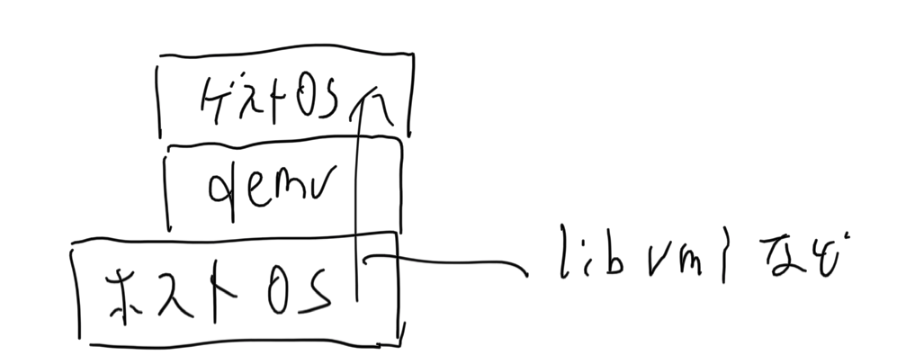
\includegraphics[bb=0 0 1000 340,width=15cm]{img/tegaki/01_vm.png}
    \end{center}
\end{figure}

\subsubsection{libvmi}

QEMUの上で実行するlibvmi\cite{osti_1334968}というものがあり.これを使用した解析も可能である.

詳しく書く

\section{RDMA}

ここにRDMAの説明をかく

\begin{figure}[htbp]
    \caption{PCI Express}
    \label{fig:zentai}
    \begin{center}
        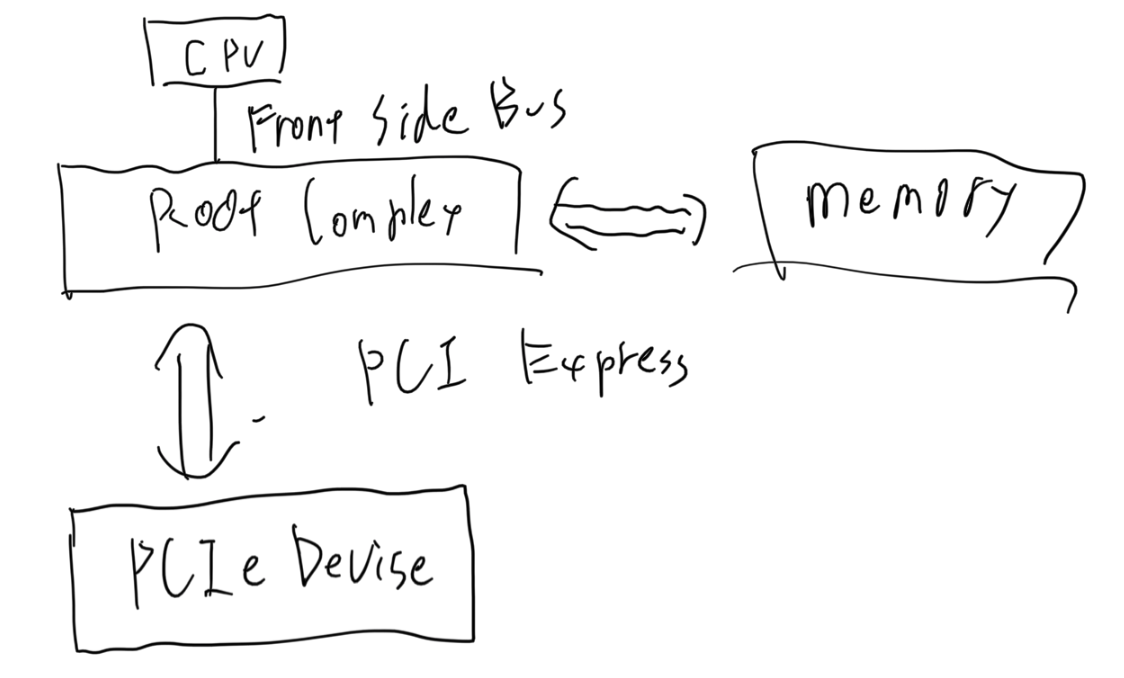
\includegraphics[bb=0 0 1000 400,width=15cm]{img/tegaki/pcie.png}
    \end{center}
\end{figure}

\subsection{InfinibandにおけるRDMA実装}

制約がかなり厳しく,本研究の用途には適さないということを書く
